%%%%%%%%%%%%%%%%%%%%%%%%%%%%%%%%%%%%%%%%%
%
% Reproducible Research Workshop Slides
% Module 04
% Perry Williams
% 09/12/2020
%
%%%%%%%%%%%%%%%%%%%%%%%%%%%%%%%%%%%%%%%%%

% ---------------------------------------------------------
%	PACKAGES AND THEMES
% ---------------------------------------------------------

\documentclass{beamer}\usepackage[]{graphicx}\usepackage[]{color}
%% maxwidth is the original width if it is less than linewidth
%% otherwise use linewidth (to make sure the graphics do not exceed the margin)
\makeatletter
\def\maxwidth{ %
  \ifdim\Gin@nat@width>\linewidth
    \linewidth
  \else
    \Gin@nat@width
  \fi
}
\makeatother

\usepackage{Sweavel}



\usetheme{Madrid}
\usecolortheme{beaver}

\setbeamertemplate{navigation symbols}{}
\setbeamercolor{block title}{fg=black,bg=darkred}
\setbeamercolor{block body}{fg=black,bg=lightgray}


\usepackage{animate}
\usepackage{booktabs}
\usepackage{graphicx}
\usepackage{mathtools}
\usepackage{mathrsfs}
\usepackage{media9}
\usepackage{listings}
\usepackage{pgf}
\usepackage{stackengine}
\usepackage{textpos}
\usepackage{tikz}
\usepackage{xcolor}
\lstset{breaklines=true} % break long lines
\newcommand\Fontvi{\fontsize{14}{7.2}\selectfont}
\newcommand{\backupbegin}{
  \newcounter{finalframe}
  \setcounter{finalframe}{\value{framenumber}}
}
\newcommand{\backupend}{
  \setcounter{framenumber}{\value{finalframe}}
}
\renewcommand\useanchorwidth{T}
\def\theyearwidth{1.5pt}
\newlength\yrsfboxrule
\yrsfboxrule .4\fboxrule
\newcommand\yearwidth[1]{\def\theyearwidth{#1}\ignorespaces}
\newcommand\skipyears[2][white]{%
  \fboxrule\yrsfboxrule%
  \fboxsep=-\yrsfboxrule%
  \fcolorbox{gray}{#1}{\strut\hspace{#2}}%
  \ignorespaces%
}
\newcommand\showyear[2][black]{%
  \fboxsep=0pt%
  \stackon{%
    \colorbox{#1}{\strut\hspace{\theyearwidth}}
  }{\sffamily\small#2}%
  \ignorespaces%
}

\let\svthefootnote\thefootnote
\textheight 1in
\newcommand\blankfootnote[1]{%
  \let\thefootnote\relax\footnotetext{#1}%
  \let\thefootnote\svthefootnote%
}
\usetikzlibrary{fadings}
\tikzfading[name=fade out, inner color=transparent!0,
         outer color=transparent!100]

\graphicspath{{./Images/}}

% ---------------------------------------------------------
%	TITLE PAGE
% ---------------------------------------------------------

\title[Reproducible Research]{\normalsize GRAD 778: Reproducible Research}
\author[Perry Williams]{\footnotesize Perry J. Williams}
\vspace{1in}
\institute[]{
  Department of Natural Resources and Environmental Science\\
  University of Nevada, Reno}
\date[\today]{\today}
\begin{document}

\begin{frame}
\begin{textblock*}{4cm}(8cm,5.8cm) % {block width} (coords)
      \begin{tikzpicture} \path (0,0) rectangle
        (5,7); \node[scope fading=fade out,inner
        sep=0pt,outer sep=0pt,anchor=south east]
        at(5,5)
        {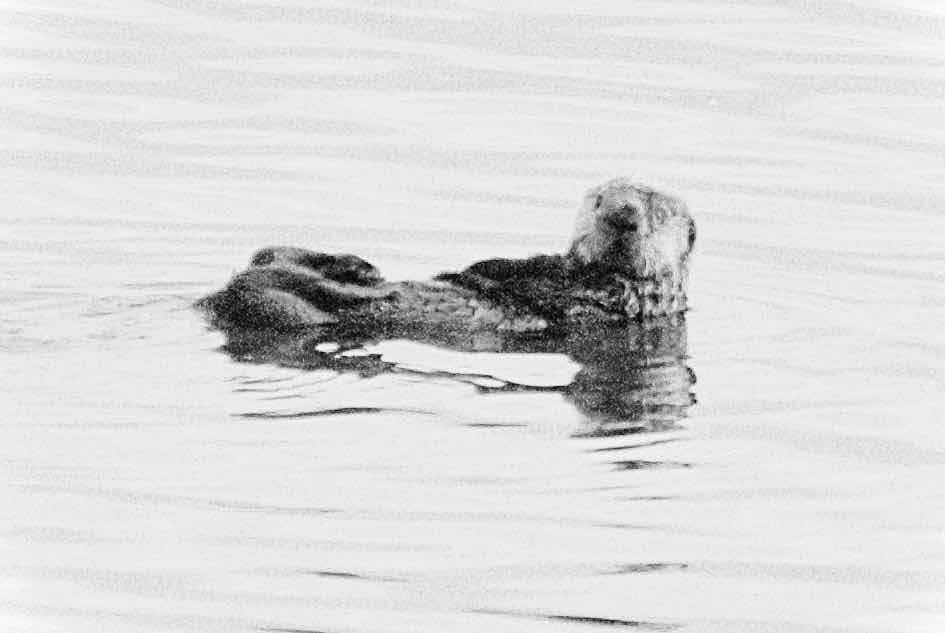
\includegraphics[width=5cm]{icon2}};
      \end{tikzpicture}
  \end{textblock*}
\begin{textblock*}{4cm}(-2cm,5.5cm) % {block width} (coords)
      \begin{tikzpicture} \path (0,0) rectangle
        (5,7); \node[scope fading=fade out,inner
        sep=0pt,outer sep=0pt,anchor=south east]
        at(5,5)
        {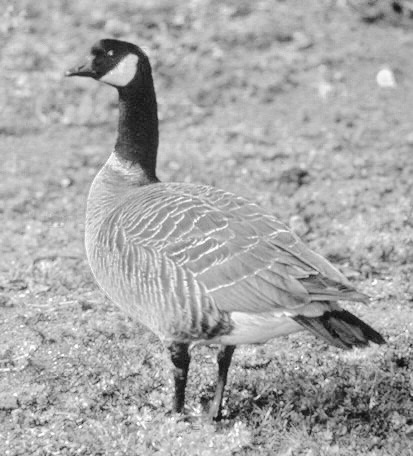
\includegraphics[width=3cm]{cago3}};
      \end{tikzpicture}
  \end{textblock*}
  \titlepage
\end{frame}

% -------------------------------------------------------
% PRESENTATION SLIDES
% -------------------------------------------------------

% ------------------------------------------------
\section{Using \texttt{knitr}}
% ------------------------------------------------

\begin{frame}[noframenumbering]
  \begin{center}
      \textsc{\textrm{Using}} \texttt{knitr}
  \end{center}
\end{frame}

\begin{frame}{What \texttt{knitr} Does}
  \begin{itemize}
  \item \texttt{knitr} ties together your presentation of results with the creation of those results
  \item Choose a mark-up code. We focus on \LaTeX in this workshop (an alternative is Markdown)
  \item Write document with mark-up code, with \texttt{R} chunks embedded in mark-up code.
  \item \texttt{knitr} converts \texttt{R} chunks to mark-up language (this would be tedious without \texttt{knitr})
  \item We can then compile final mark-up code using appropriate compiler
  \end{itemize}
\end{frame}

\begin{frame}
   \begin{center}
     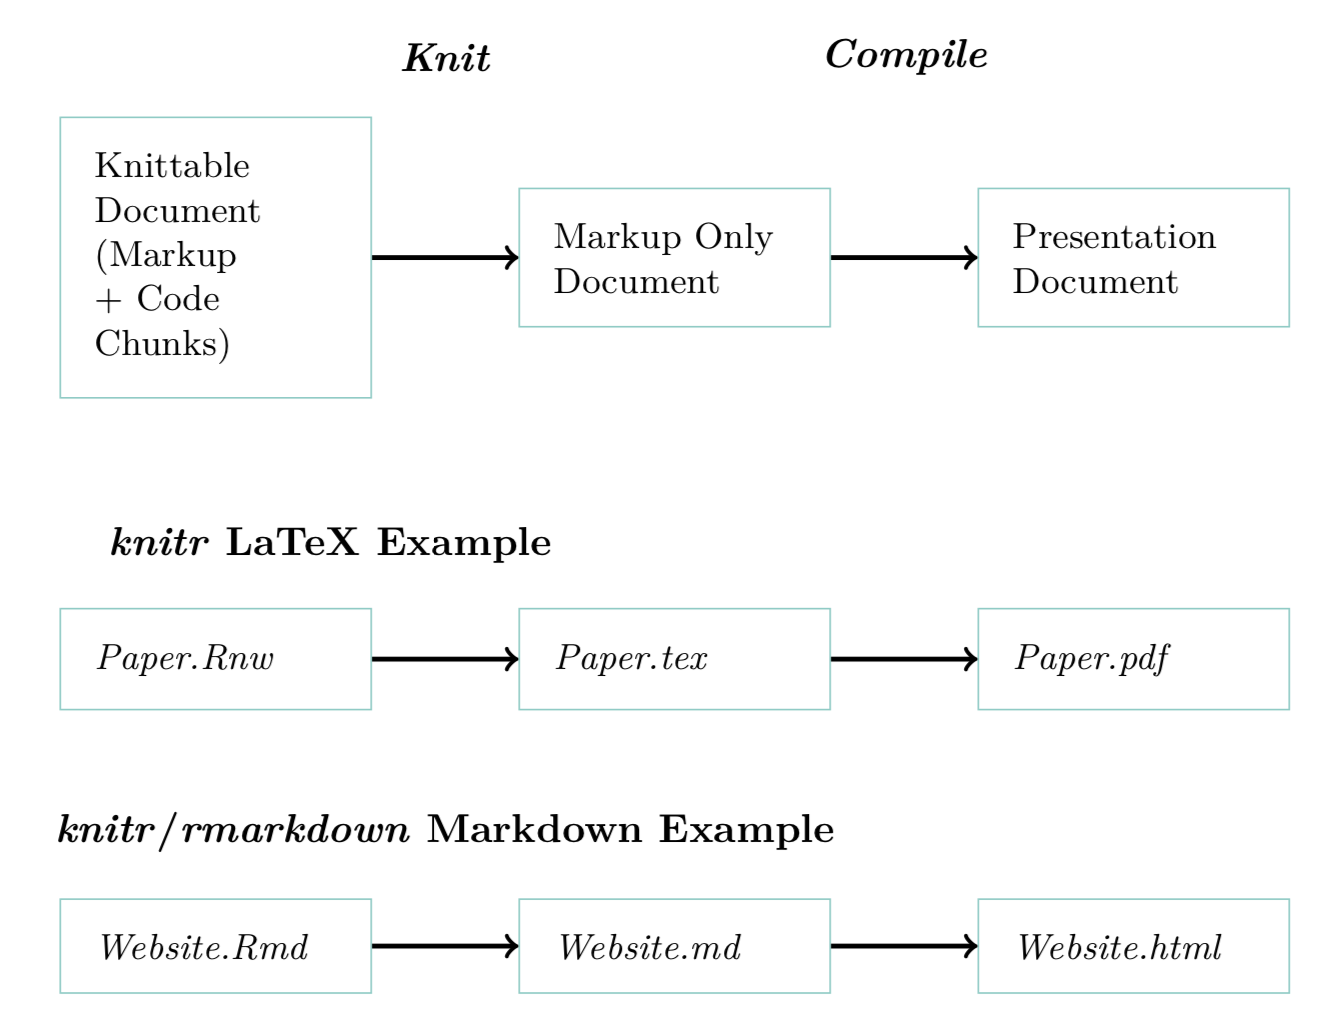
\includegraphics[width=.9\linewidth]{knitrprocess}
   \end{center}
 \end{frame}

\begin{frame}
   \begin{columns}
     \begin{column}{0.5\textwidth}
       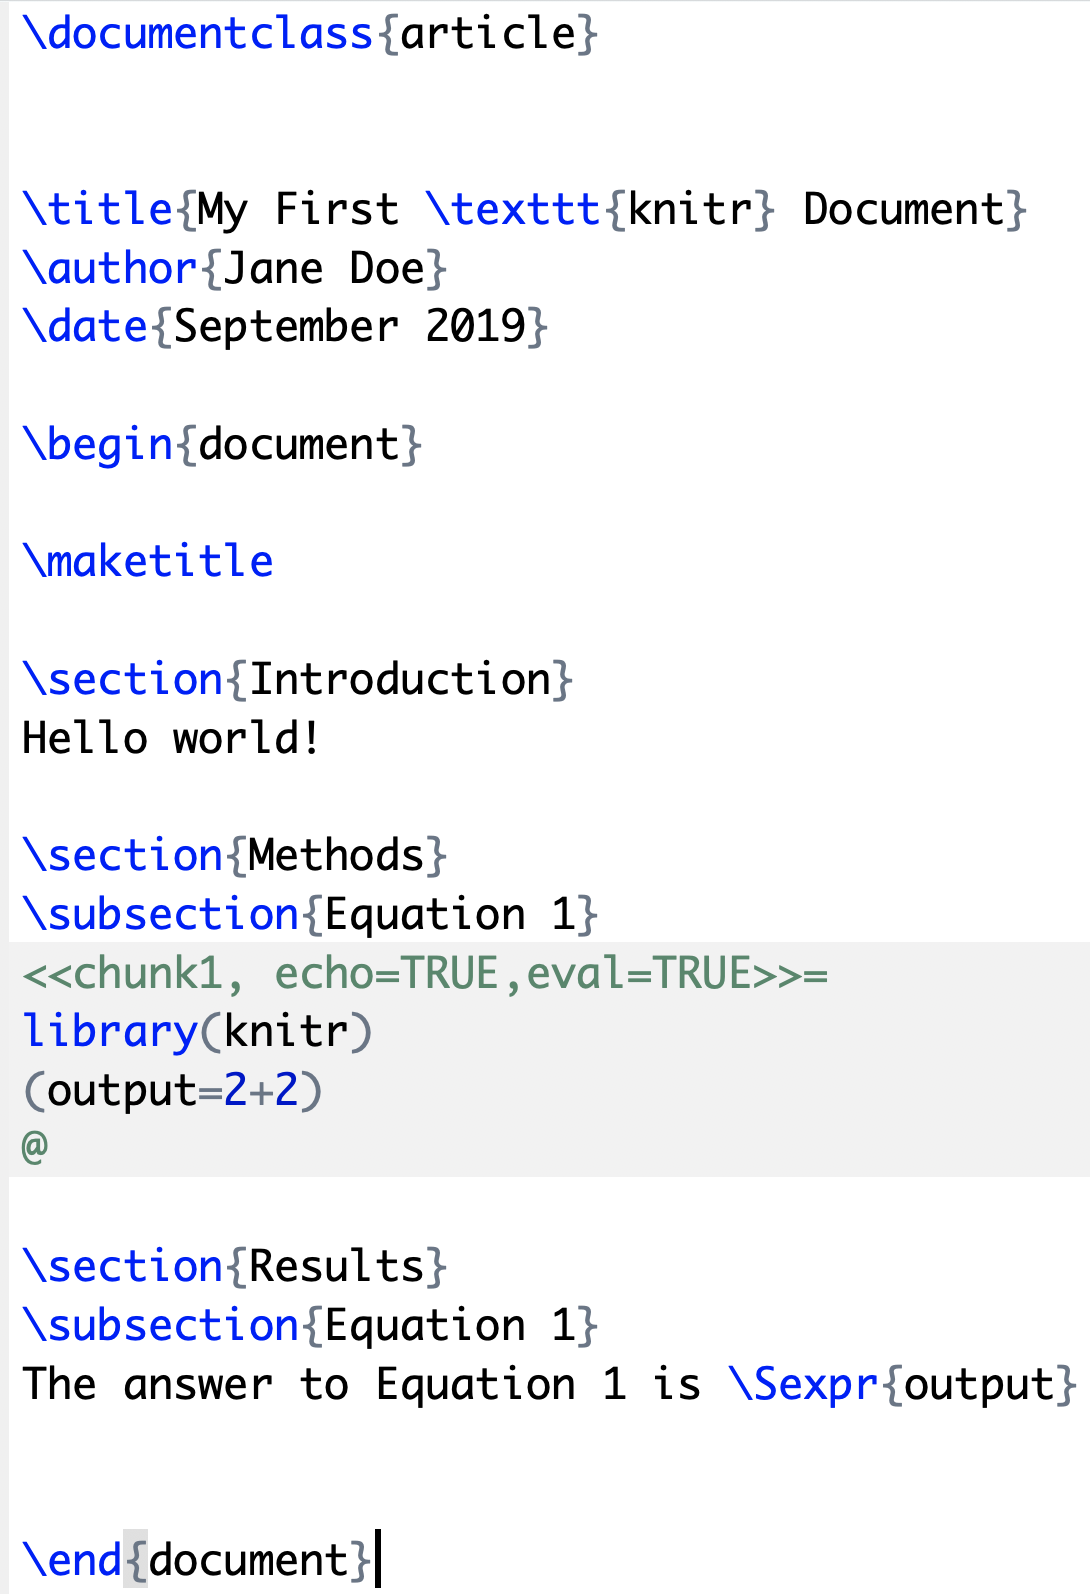
\includegraphics[width=.8\linewidth,keepaspectratio]{knitr1a}
      \end{column}
      \begin{column}{0.5\textwidth}
        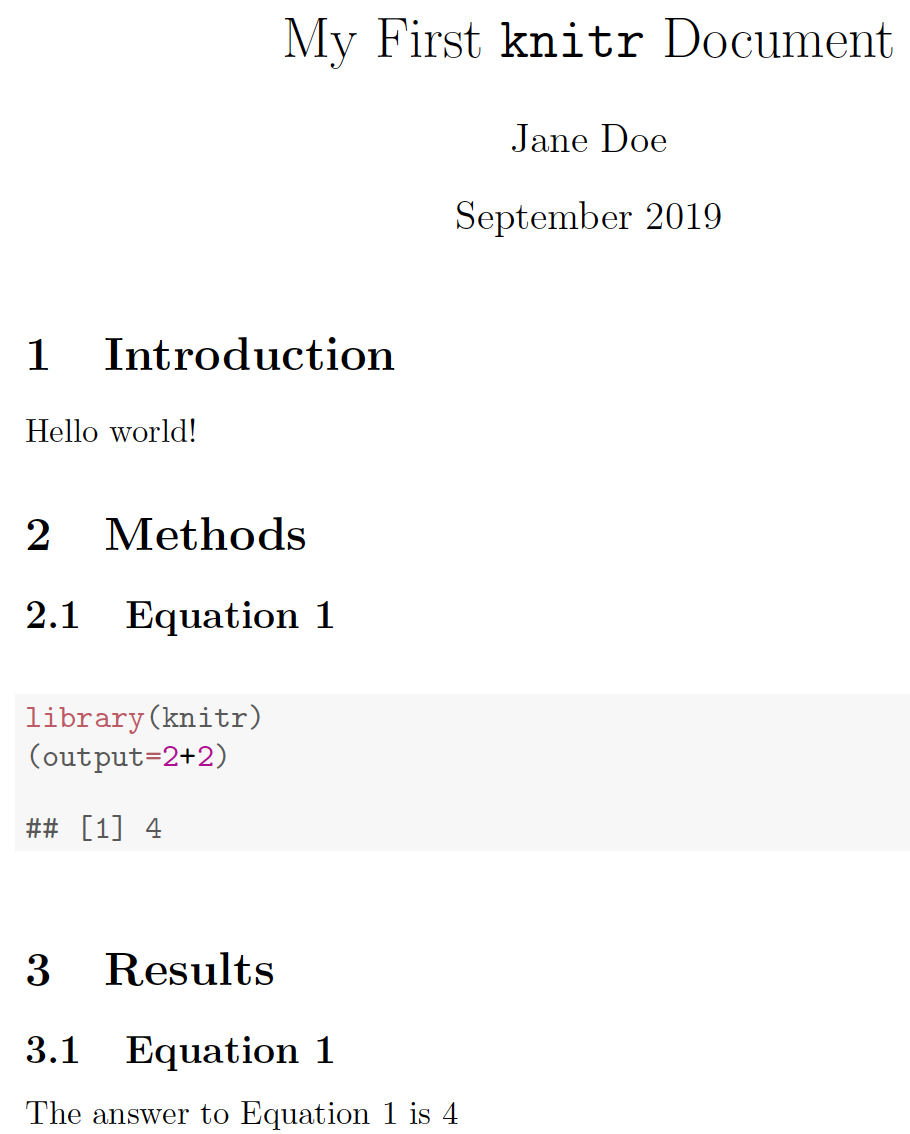
\includegraphics[width=.8\linewidth,keepaspectratio]{knitr1b}
      \end{column}
    \end{columns}
\end{frame}

\begin{frame}
   \begin{center}
     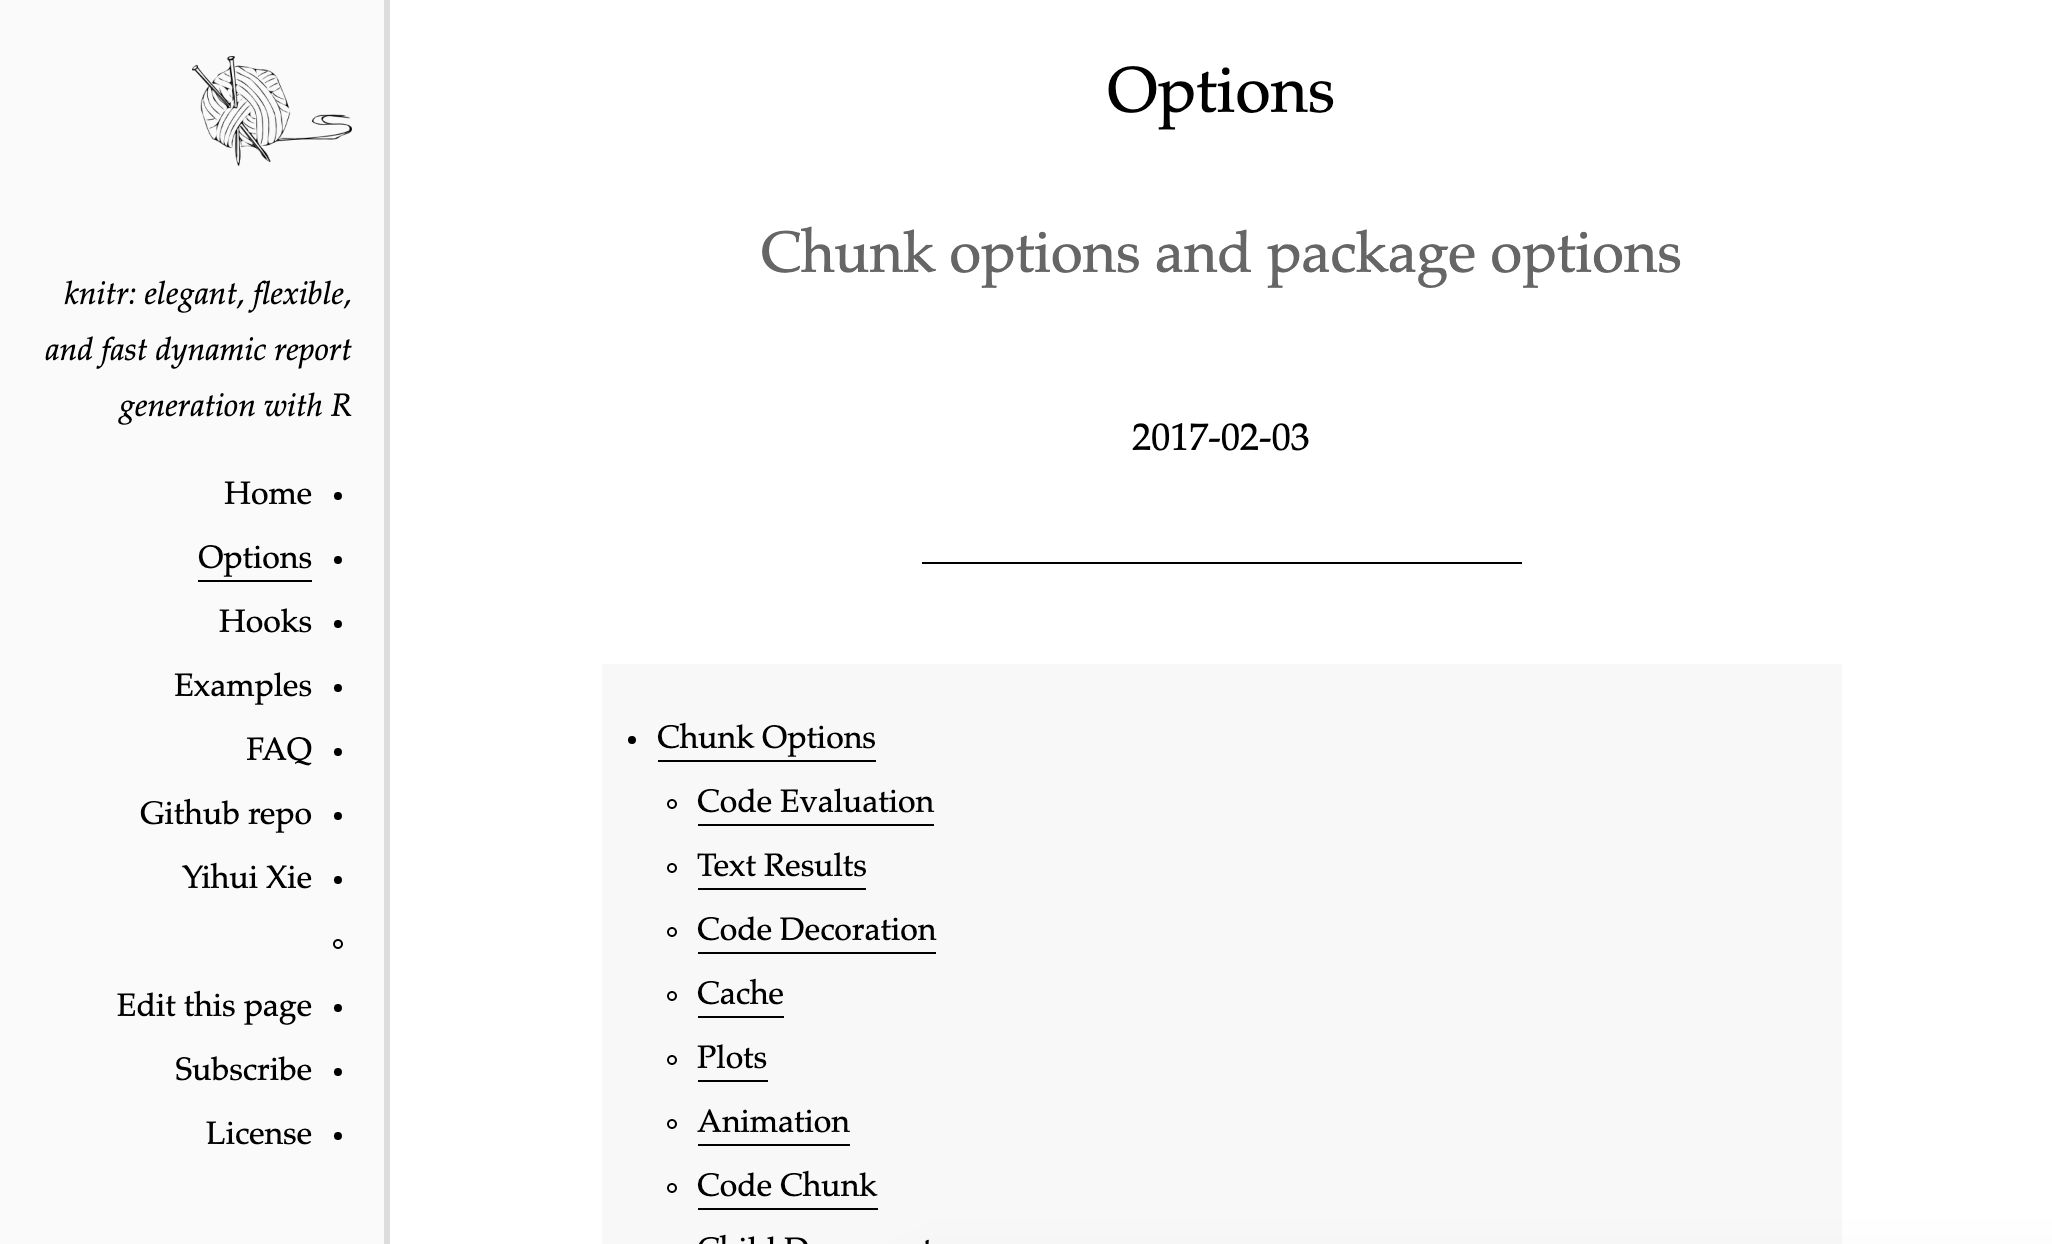
\includegraphics[width=.9\linewidth]{chunkoptions}
   \end{center}
\end{frame}


\begin{frame}{Second \texttt{knitr} document}

\end{frame}

\begin{frame}[t]{Exercise 2}
\textbf{Create an interactive \texttt{knitr} document that:}
\begin{itemize}
\item includes the analysis \texttt{MainAnalysis.R} within the \texttt{.Rnw} document,
\item replaces all static values (e.g., parameter estimates, figure and table numbers) with dynamic values from the incorporated analysis,
\item permits you to change the data in the analysis (i.e., remove Alaska), and automatically updates the parameter values.
\end{itemize}
\end{frame}


\end{document}


